\section{Grappa}
Existing shared memory applications typically do fine-grained operations on data, assuming it is all cheap to access.
Naively translating these applications to PGAS languages often results in poor performance because many operations must then be done via fine-grained remote communication.
Much research has been done to improve performance of PGAS implementations by coming up with better ways to partition data and schedule computation, and do communication in bulk to best utilize network resources.
For regular workloads, most pointedly dense linear algebra, much of this can now be automatically optimized generically.

Irregular applications, on the other hand, are characterized by being highly dependent on the shape of the data, making it difficult to statically partition, causing load imbalance, and requiring a majority of fine-grained random accesses. The goal of the Grappa runtime is to provide a PGAS implementation that has been designed from the ground up to handle such applications.

\begin{figure}[ht]
  \centering
  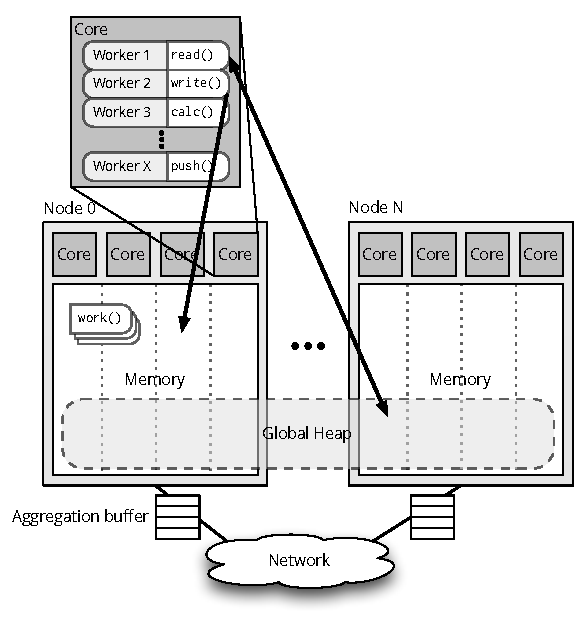
\includegraphics[width=0.5\textwidth]{figs/grappa_system.pdf}
  \caption{Grappa System Overview: Global address space is partitioned among all nodes, each core owns a portion, and with a portion devoted to the linearly-addressable global heap. Thousands of workers multiplexed onto each core, context switching to tolerate long-latency remote operations.}
  \label{fig:system}
\end{figure}

\subsection{Tasks}
\TODO{describe how tasks work}

\subsection{Global Memory}
\TODO{explain how memory is partitioned}

\subsection{Communication}
\TODO{remote delegate operations, aggregation}
